% Sources: the author's literature session, 2026-11-19 (table as supplied); figure: figures/plot_mass_comparison.py

\section{Published mass estimates}
\label{app:masses}

Table~\ref{tab:masses} collects the published estimates of the mass of the compact object in the sources of Table~\ref{tab:sources}.
Figure~\ref{fig:masses} compares them with the mass of the best BH fit of each source (Table~\ref{tab:bestfit_params} and Fig.~\ref{fig:chi2_overview}).
% OUTLINE (author): what the comparison shows.

\begin{table*}
\centering
\caption{Published estimates of the compact-object mass $M_{\rm X}$. ``n.m.'': not measured.
$a$: dimensionless BH spin. For Holmberg~IX X-1, $\hat M \equiv \alpha M_{\rm X}/M_\odot$ with $1/6 \le \alpha < 1$.}
\label{tab:masses}
\footnotesize
\begin{tabular}{@{}lp{0.13\textwidth}p{0.19\textwidth}p{0.26\textwidth}p{0.15\textwidth}@{}}
\toprule
Code name & Identification & $M_{\rm X}$ & Method & References \\
\midrule
HolmII & Holmberg~II X-1 & $16$--$36\,M_\odot$ & onset of spectral deviations taken as the Eddington or supercritical rate & \citealt{Barra2024} \\
 & & $16$--$70\,M_\odot$ & combined range quoted from \citet{Barra2024, ReyeroSerantes2024} & \citealt{Fogantini2026} \\
 & & $\geq 25\,M_\odot$ & radio jet power & \citealt{Cseh2014} \\
HolmIX & Holmberg~IX X-1 & $4 \lesssim \hat M \lesssim 10$ & disc--corona fit, optical/UV to X-ray & \citealt{Gill2021} \\
M101ULS & M101 ULX-1 & $20$--$30\,M_\odot$ ($\geq 5\,M_\odot$) & radial velocity of a Wolf--Rayet donor, $P_{\rm orb} = 8.2$~d; disputed & \citealt{Liu2013} \\
 & & $(3.2$--$4.3)\times10^{4}\,M_\odot$ & scaling of the $\Gamma$--$\dot M$ correlation & \citealt{Titarchuk2016} \\
M51ULS & M51 ULX-7\idq{} & NS, n.m. & companion mass $\geq 8.3\,M_\odot$ for $M_{\rm NS} = 1.4\,M_\odot$, from the pulse-timing orbital solution & \citealt{RodriguezCastillo2020} (also pulsations) \\
M81ULS & M81 X-6\idq{} & NS candidate, n.m. & -- & \citealt{Amato2023} \\
NGC1313B & NGC~1313 X-1\idq{} & ${\approx}\,5000\,M_\odot$ & 3:2 QPO frequency scaling & \citealt{Pasham2015} \\
 & & $2524$--$6811\,M_\odot$ & sub-Eddington IMBH (Huang 2019, as quoted) & \citealt{Majumder2023} \\
 & & $275$--$2283\,M_\odot$ ($a=0$); $92$--$883\,M_\odot$ ($a=0.99$) & QPO frequency and $L_{\rm bol}$ fitted with shock-induced accretion solutions & \citealt{Majumder2023} \\
NGC1313H & NGC~1313 X-2\idq{} & NS, n.m. & -- & pulsations: \citealt{Sathyaprakash2019} \\
NGC247S, NGC247SS & NGC~247 ULX-1 & $600$--$3000\,M_\odot$ ($a=0$, face-on; larger otherwise) & disc inner radius set to the innermost stable orbit, thermal state & \citealt{Jin2011} \\
NGC300 & NGC~300 ULX-1 & NS, n.m. & $M_{\rm X} = 1.4$--$2.0\,M_\odot$ assumed & \citealt{Heida2019}; pulsations: \citealt{Carpano2018} \\
NGC5408 & NGC~5408 X-1 & $1000$--$9000\,M_\odot$ & QPO frequency--spectral index scaling; conservative range, $2000$--$5000\,M_\odot$ more likely & \citealt{StrohmayerMushotzky2009} \\
 & & $\gtrsim 800\,M_\odot$ & lower limit, same method, if only the saturated part of the relation is observed & \citealt{Pasham2012} \\
 & & $207$--$1851\,M_\odot$ ($a=0$); $104$--$635\,M_\odot$ ($a=0.99$) & QPO frequency and $L_{\rm bol}$ fitted with shock-induced accretion solutions & \citealt{Majumder2023} \\
NGC55 & NGC~55 ULX-1 & $6$--$14\,M_\odot$ & onset of spectral deviations taken as the Eddington or supercritical rate & \citealt{Barra2022} \\
NGC6946 & NGC~6946 X-1 & $(1$--$4)\times10^{3}\,M_\odot$ & mHz QPO taken as type-C, scaled to GRS~1915+105 ($14\,M_\odot$) & \citealt{Rao2010} \\
 & & $130$--$1300\,M_\odot$ & break frequency scaled to Cyg~X-1 & \citealt{Rao2010} \\
 & & $248$--$2221\,M_\odot$ ($a=0$); $214$--$696\,M_\odot$ ($a=0.99$) & QPO frequency and $L_{\rm bol}$ fitted with shock-induced accretion solutions & \citealt{Majumder2023} \\
NGC7793 & NGC~7793 P13 & NS, n.m.; $M_{\rm X} < 15\,M_\odot$ & X-ray heating of the B9Ia donor, $P = 64$~d, BH assumed & \citealt{Motch2014}; pulsations: \citealt{Furst2016, Israel2017} \\
\bottomrule
\end{tabular}
% pulsation references as in tab:sources (author 2026-11-19)
% source: web search 2026-11-19; every value checked 2026-11-24 against the papers' texts (arXiv) and every reference against ADS
%         by another session (report passed by the author). Huang 2019 value taken from Majumder2023, original not checked.
%         Majumder2023 = arXiv:2309.11182 = 2023MNRAS.526.2086M (confirmed). Changed 2026-11-24: Majumder2023 method (was
%         "spectral modelling"), Jin2011 method and range (was ">= 600 Msun, T_in ~ M^-1/4"), M51 companion mass for 1.4 Msun NS,
%         Strohmayer & Mushotzky likely range, Pasham2012 condition, Rao2010 type-C reference and break-frequency estimate.
% VERIFY: Huang 2019 (NGC 1313 X-1) is cited only as quoted in Majumder2023; the literature session does not have the
%         original paper. Send it the PDF to make it an entry of its own.
% VERIFY: Gill2021: only the arXiv version was found; if it has been published in a journal, update its journal field.
\end{table*}

\begin{figure}
\centering
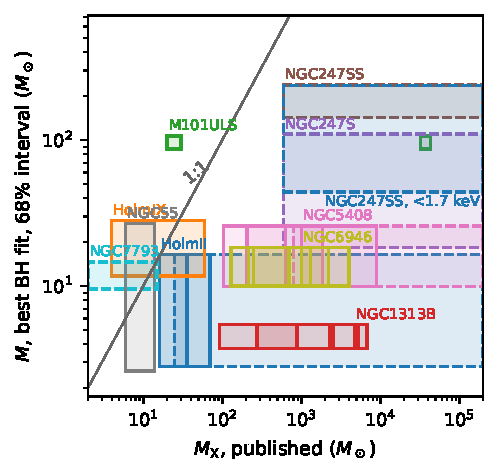
\includegraphics[width=\columnwidth]{mass_comparison.pdf}
\caption{Mass of the best BH fit of each source (68\% posterior interval, vertical extent) against the published estimates of Table~\ref{tab:masses} (horizontal extent), one rectangle per estimate.
Dashed outlines are limits, which run to the edge of the plot.
The single value of NGC1313B (${\approx}5000\,M_\odot$) is drawn $\pm5$\%.
{The range of \citet{Jin2011} for NGC~247 ULX-1, $600$--$3000\,M_\odot$ for a non-spinning BH seen face-on, is drawn as a lower limit, because spin or a tilted disc would raise it.}
For Holmberg~IX X-1 the published range is $\hat M/\alpha = 4$--$60\,M_\odot$.
Sources with no published mass are not shown; the line is $1{:}1$.}
\label{fig:masses}
\end{figure}
% figure: this repository, figures/plot_mass_comparison.py (layout: the author's sketch 2026-11-19; 2026-11-24: Rao2010 break-frequency
%         estimate added, Pasham2012 label); fits: set "BH" of
%         ULXspectra-mc summaries/best_refit_per_source.tsv (e597ba3), NGC247S BH3a; for the NS sources and NGC1313B the
%         best BH fit is not their best fit overall (Fig. chi2_overview)
